% vim: set tw=0:
\documentclass{beamer}
\usepackage{graphicx}

% Reasonable themes:
% Antibes Bergen Berkeley Berlin Frankfurt Goettingen Ilmenau Luebeck Malmoe
% Montpellier PaloAlto Rochester Singapore Szeged Warsaw bars boxes
% compatibility default lined plain shadow sidebar split tree
% And these ones include the author's name on every slide:
% Berkeley

% Declare themes.
\mode<presentation>
\usetheme{UWHEP}

% Personal macros.
\newcommand{\email}[1]{{\texttt #1}}
\newcommand{\newframe}[1]{\section{#1}
    \frametitle{\sc{#1}}}
\newcommand{\subframe}[1]{\subsection{#1}
    \frametitle{\sc{#1}}}
\newcommand{\supers}[1]{\ensuremath{^\textrm{#1}}}
\newcommand{\subs}[1]{\ensuremath{_\textrm{#1}}}
\newcommand{\ca}{\ensuremath{\sim}}

% Author information.
\title{T2 Status}
\author[Maier, Mohapatra]{
    Will Maier \and Ajit Mohapatra\\ 
    {\tt wcmaier@hep.wisc.edu}\\
    {\tt ajit@hep.wisc.edu}}
\institute[Wisconsin]{University of Wisconsin - High Energy Physics}
\date{2008.12.09}
\logo{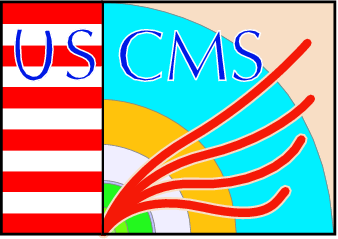
\includegraphics[height=0.6cm]{../../../Graphics/USCMS_logo.png}\hspace{.1cm}
\includegraphics[height=0.75cm]{../../../Graphics/UW_logo.png}}

\begin{document}

\begin{frame}
    \titlepage
\end{frame}

%\section{Overview}
%\begin{frame}
%    \tableofcontents
%\end{frame}

\section{Facilities}
\subsection{Software and Storage}
\begin{frame}
\frametitle{}
\begin{itemize}
    \item Three user accounts compromised; exploit attempt on login machines
    \begin{itemize}
        \item Stolen SSH keys used to access systems
        \item Rootkit found; not clear if the attempt was successful
        \item Reinstalled all login systems
        \item Notified users, scanned AFS for poorly secured SSH keys
        \item Added regular checks of SSH keys, other sensitive files
    \end{itemize}
    \item RMA several disks from new rack purchase
    \begin{itemize}
        \item 8/240 Seagate 1TB disks bad in \ca{} two months
    \end{itemize}
    \item Improved RAID monitoring on new rack
    \item Upgraded OpenAFS client on submit machines
    \begin{itemize}
        \item OpenAFS 1.4.1 would inconsistently report nanosecond values in file timestamps
        \item Confused make, breaking large software compilations
        \item Fixed in recent versions
    \end{itemize}
    \item SRM and dcap became quite slow on two separate occasions
    \begin{itemize}
        \item No indication of real cause
        \item Stopping and starting the services resolved the issue
    \end{itemize}
\end{itemize}
\end{frame}

\subsection{Production and Monitoring}
\begin{frame}
\frametitle{}
\begin{itemize}
     \item JobRobot: OK
     \item SAM: OK
     \item RSV: OK
     \item PhEDEx:
     \begin{itemize}
        \item Upgraded both Prod and Debug instances to 3\_0\_7; running Ok
        \item LoadTest is going OK with all T1s except ASGC, which we are debugging now (too many TCP streams)
        \item Usual MC data subscriptions for local users
     \end{itemize}
     \item MC Production:
     \begin{itemize}
        \item Summer08 production continues
        \item The infamous MadEvents reproduction will start later today or early tomorrow
     \end{itemize}
\end{itemize}
\end{frame}

\end{document}
